%%%%%%%%%%%%%%%%%%%%%%%%%%%%%%%%%%%%%%%%%%%%%%%%%%%%%%%%%%%%%%%%%%%%%%%%%%%%%%%%
\section{Shape-from-Shading}\label{ch:bg_sfs}
%%%%%%%%%%%%%%%%%%%%%%%%%%%%%%%%%%%%%%%%%%%%%%%%%%%%%%%%%%%%%%%%%%%%%%%%%%%%%%%%
%%%%%%%%%%%%%%%%%%%%%%%%%%%%%%%%%%%%%%%%
\begin{figure}[t]
	\centering
	\begin{subfigure}[b]{0.24\textwidth}
		\centering
		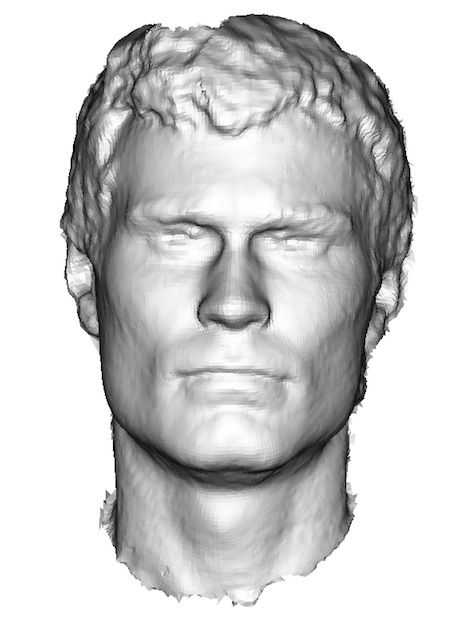
\includegraphics[height=2in]{background/images/frontal}
		\caption*{Frontal}
	\end{subfigure}
	\begin{subfigure}[b]{0.24\textwidth}
		\centering
		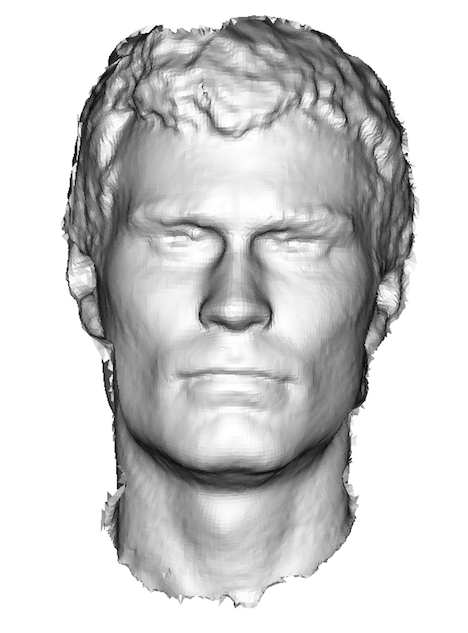
\includegraphics[height=2in]{background/images/invert}
		\caption*{Inverted}
	\end{subfigure}
	\begin{subfigure}[b]{0.24\textwidth}
		\centering
		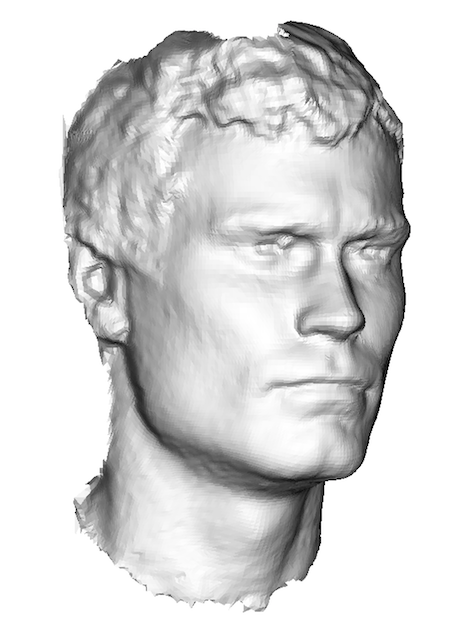
\includegraphics[height=2in]{background/images/frontal_rotate}
		\caption*{Frontal}
	\end{subfigure}
	\begin{subfigure}[b]{0.24\textwidth}
		\centering
		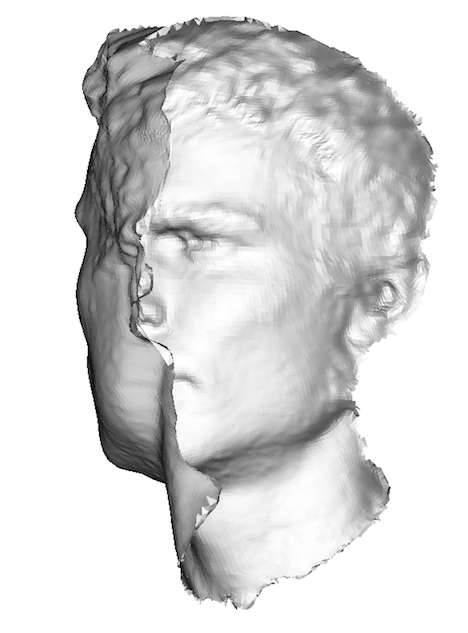
\includegraphics[height=2in]{background/images/invert_rotate}
		\caption*{Inverted}
	\end{subfigure}
	\caption{An example of a bas-relief ambiguity for a mesh illuminated
	         frontally with a lambertian shader. ``Inverted'' implies
	         that the mesh is actually facing away from the camera and thus
	         the interior is visible, as demonstrated by the rotated
	         ``Inverted'' image. Both of the non-frontal images are rotated
	         versions of the frontal images, approximately $25^\circ$ around
	         the Yaw axis.}
\label{fig:sfs_bas_relief}
\end{figure}
%%%%%%%%%%%%%%%%%%%%%%%%%%%%%%%%%%%%%%%%
Shape-from-shading (SfS) is the process of attempting to recover surface
information from an object in an image using \textit{inverse rendering}, 
or \textit{image formation}, methods. The primary assumption is that shading, or
the intensity of a pixel in the image, is generated as a function of the surface
geometry and its interaction with light reflected off the surface and captured
by an imaging device. Naturally, the reality of this process in the physical
world is a complex interaction between light and both microscopic and
macroscopic elements of the surface structure. This is further complicated by
the noise present in the recording procedure of the camera sensing
hardware. Furthermore, it is well known that shading alone is insufficient to
disambiguate shape. For example, the well known bas-relief
ambiguity~\cite{belhumeur1999bas} is demonstrated for a facial mesh in
\cref{fig:sfs_bas_relief}. The bas-relief ambiguity states that for an object
imaged under orthographic projection that exhibits lambertian reflectance, there
exists a family of transformations (generalized bas-relief transformations) for
which the images produced will be identical. In fact, more generally there
exists an infinite number of ways to describe any image given only shading
information through different arrangements of surfaces, lightings and
albedos~\cite{adelson1996perception}. However, despite the ill-posedness of the
SfS problem, shading does in fact provide a very strong imaging prior and many
higher frequency detail such a wrinkles can only be recovered using shading
cues. Therefore,
%%%%%%%%%%%%%%%%%%%%%%%%%%%%%%%%%%%%%%%%%%%%%%%%%%%%%%%%%%%%%%%%%%%%%%%%%%%%%%%%
